\documentclass[a4paper,12pt]{ltjsarticle}
\usepackage[top=25mm,bottom=25mm,left=25mm,right=25mm]{geometry}
\usepackage{graphicx}
\usepackage{float}
\usepackage{booktabs}
\usepackage{array}
\usepackage{enumitem}
\usepackage{hyperref}
\usepackage{caption}

\begin{document}

\begin{center}
  {\Large \textbf{第2回議事録}}\\[8pt]
  {\large チーム4}
\end{center}

\vspace{4mm}

%-------------------------------------------------------------------
\section*{1.基本情報}
\begin{tabular}{ll}
  \toprule
  日時     & 2026年4月22日（水） \\
  会議場所 & 731教室 \\
  目的     & プロジェクト計画の作成 \\
  チーム番号 & 4 \\
  議事録作成者 & 酒井睦基 \\
  \bottomrule
\end{tabular}

\vspace{4mm}
\noindent\textbf{参加者}

\begin{tabular}{ll}
  2年 & 山口汐里，佐藤夏美，成毛海人 \\
  3年 & 細澤悠真，武本龍，酒井睦基 \\
\end{tabular}

%-------------------------------------------------------------------
\section*{2.議題一覧}
\begin{enumerate}[label=議題\arabic*：]
  \item 目標を達成するための案
  \item 有効指標 MOE
  \item FBS と PBS の原案
  \item WBS と役割分担の原案
  \item 個人ごとの次回までに実施する内容
\end{enumerate}

%-------------------------------------------------------------------
\section*{3.議題ごとの内容}

\subsection*{議題①：目標を達成するための案}

\subsubsection*{社会的背景の決定}
\begin{itemize}
  \item 山口・佐藤・酒井：通信技術に関する技術的課題を提案 → 社会的背景が普遍的でなく代替も見つからなかったため\textbf{却下}
  \item 成毛：聴覚障がい者にシフトした社会的背景を提案 → 定量的評価の定義が難しいため\textbf{却下}
  \item 武本：大学生の急性ストレス軽減を目的とした社会的背景を提案 → 社会的背景・既存技術・解決手法・評価指標の妥当性を検討した結果，\textbf{本提案手法に決定}
  \item 細澤：入眠サポートを目的とした社会的背景を提案 → 評価指標が客観的な定性情報となってしまうため\textbf{却下}
\end{itemize}

\subsubsection*{プロジェクトの全体像とゴール}
\begin{description}
  \item[開発するシステム]
    3つの異なる楽器「クラリネット」「フルート」「オルガン」をメイン楽器として，「パーカッション」をリズム楽器とするオーケストレーションで「きらきら星」の演奏を行うシステム
  \item[最終的なゴール]
    輪唱曲が演奏できる（曲の識別が可能な精度）
\end{description}

\subsubsection*{成果物の定義（完成条件）}
\begin{description}
  \item[最低限達成すべき機能]~
    \begin{itemize}
      \item 各楽器の音を識別できるレベルの演奏機能
      \item 輪唱曲として判別可能な同期精度
      \item リラクゼーションアニメーション
    \end{itemize}
  \item[追加機能（可能であれば）]~
    \begin{itemize}
      \item 可変テンポ調整機能
      \item 楽器の音量調整機能
      \item 音の強弱調整機能
      \item エンターテイメント機能（未定）
    \end{itemize}
  \item[動作確認の方法]~
    \begin{itemize}
      \item 同期：LED ライト点滅で送受信の確認が取れること
      \item 楽器：それぞれの楽器音が出せること（波形確認と主観的な聴認）
      \item 結合：楽器を4つ合わせて動作可能かどうかを確認
    \end{itemize}
\end{description}

\subsubsection*{決定事項}
3つの異なる楽器「クラリネット」「フルート」「オルガン」をメイン楽器として，「パーカッション」をリズム楽器とするオーケストレーションで「きらきら星」の演奏を行うシステムに決定した．

\subsubsection*{保留・次回検討事項}
\begin{itemize}
  \item エンターテインメント性の内容（保留）
  \item 全体のシステムの構成（次回検討）
\end{itemize}

%-------------------------------------------------------------------
\subsection*{議題②：有効指標MOEの決定}

\begin{figure}[H]
  \centering
  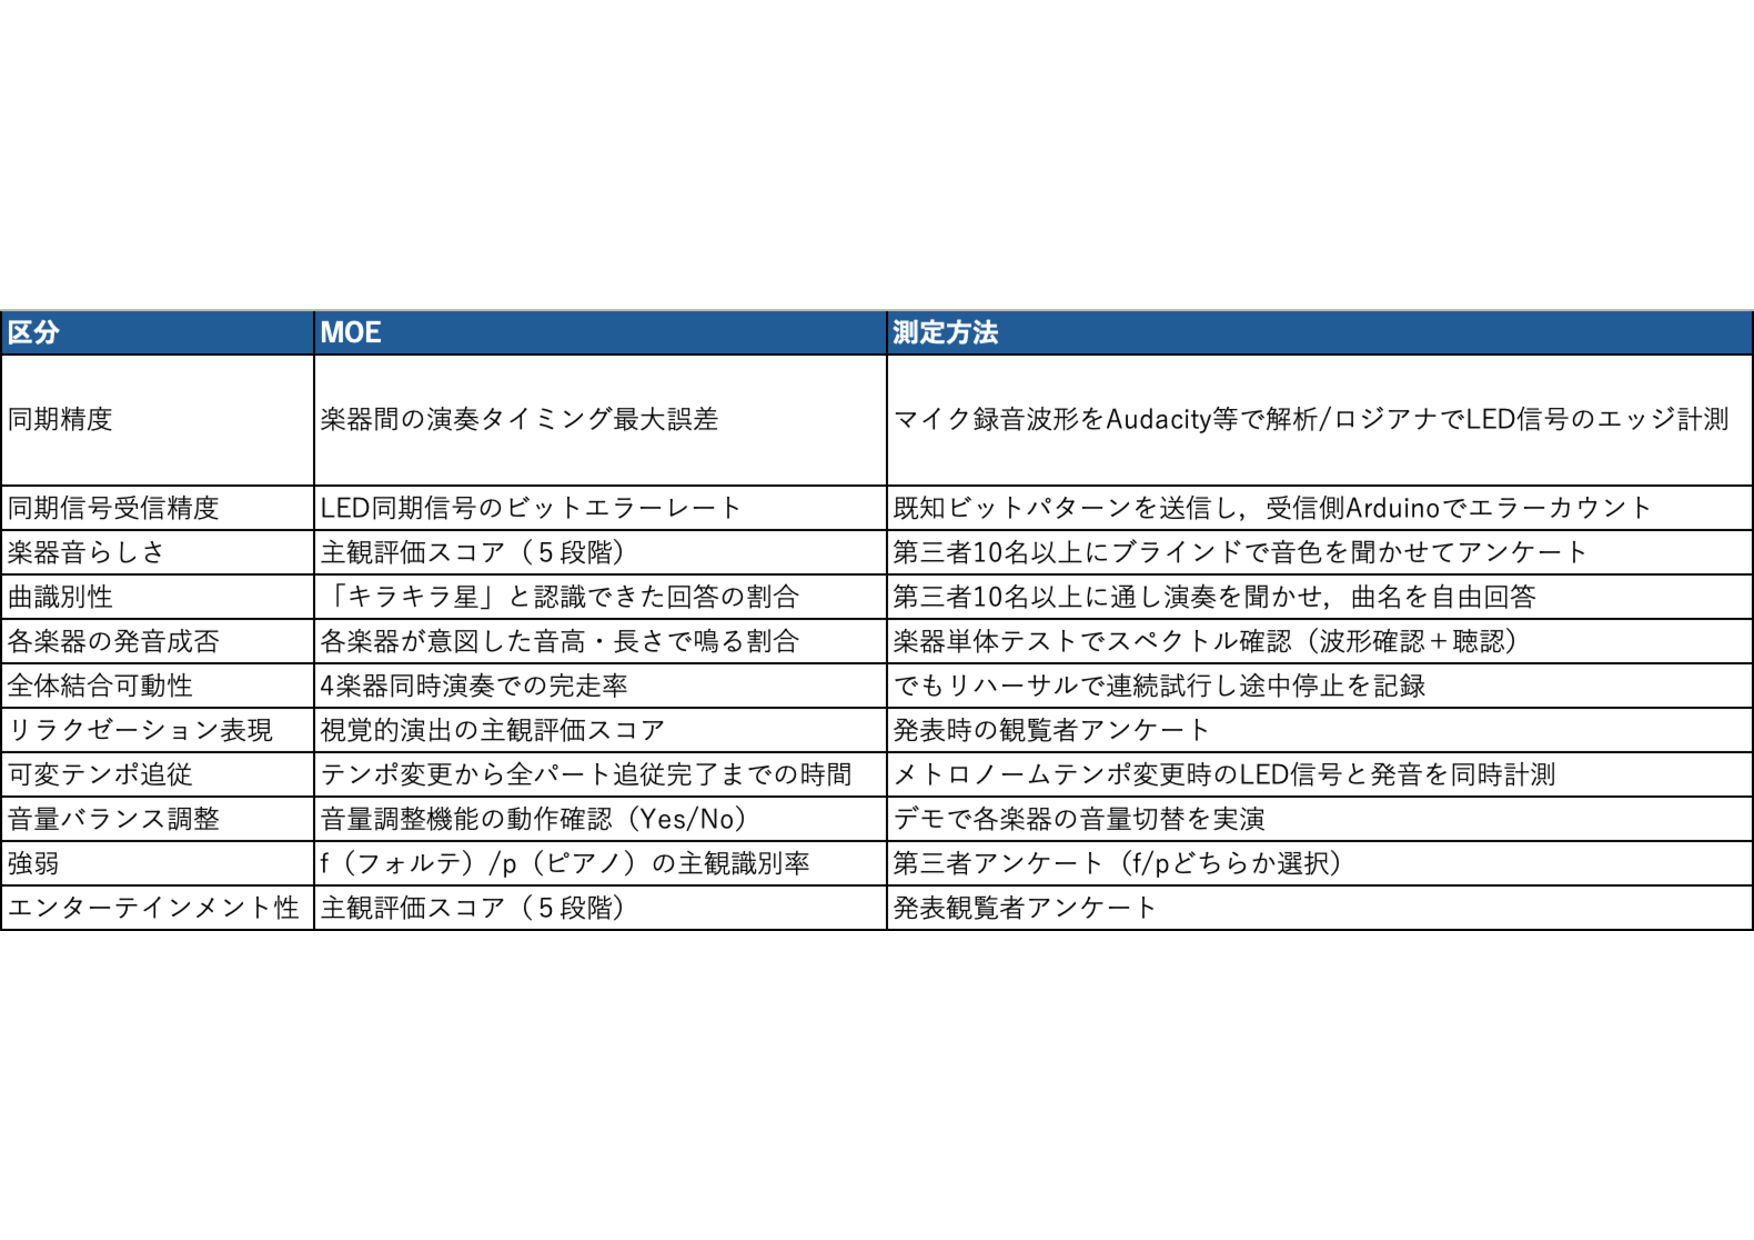
\includegraphics[width=1.0\textwidth]{fig/hck_moe.pdf}
  \caption{MOEの原案}
  \label{fig:moe}
\end{figure}

\begin{description}
  \item[ToDo / アクション] 各 MOE の目標値の調査
  \item[次回検討事項] MOE の確認・修正・確定
\end{description}

%-------------------------------------------------------------------
\subsection*{議題③：FBS と PBS の原案}

\subsubsection*{FBS}
\begin{figure}[H]
  \centering
  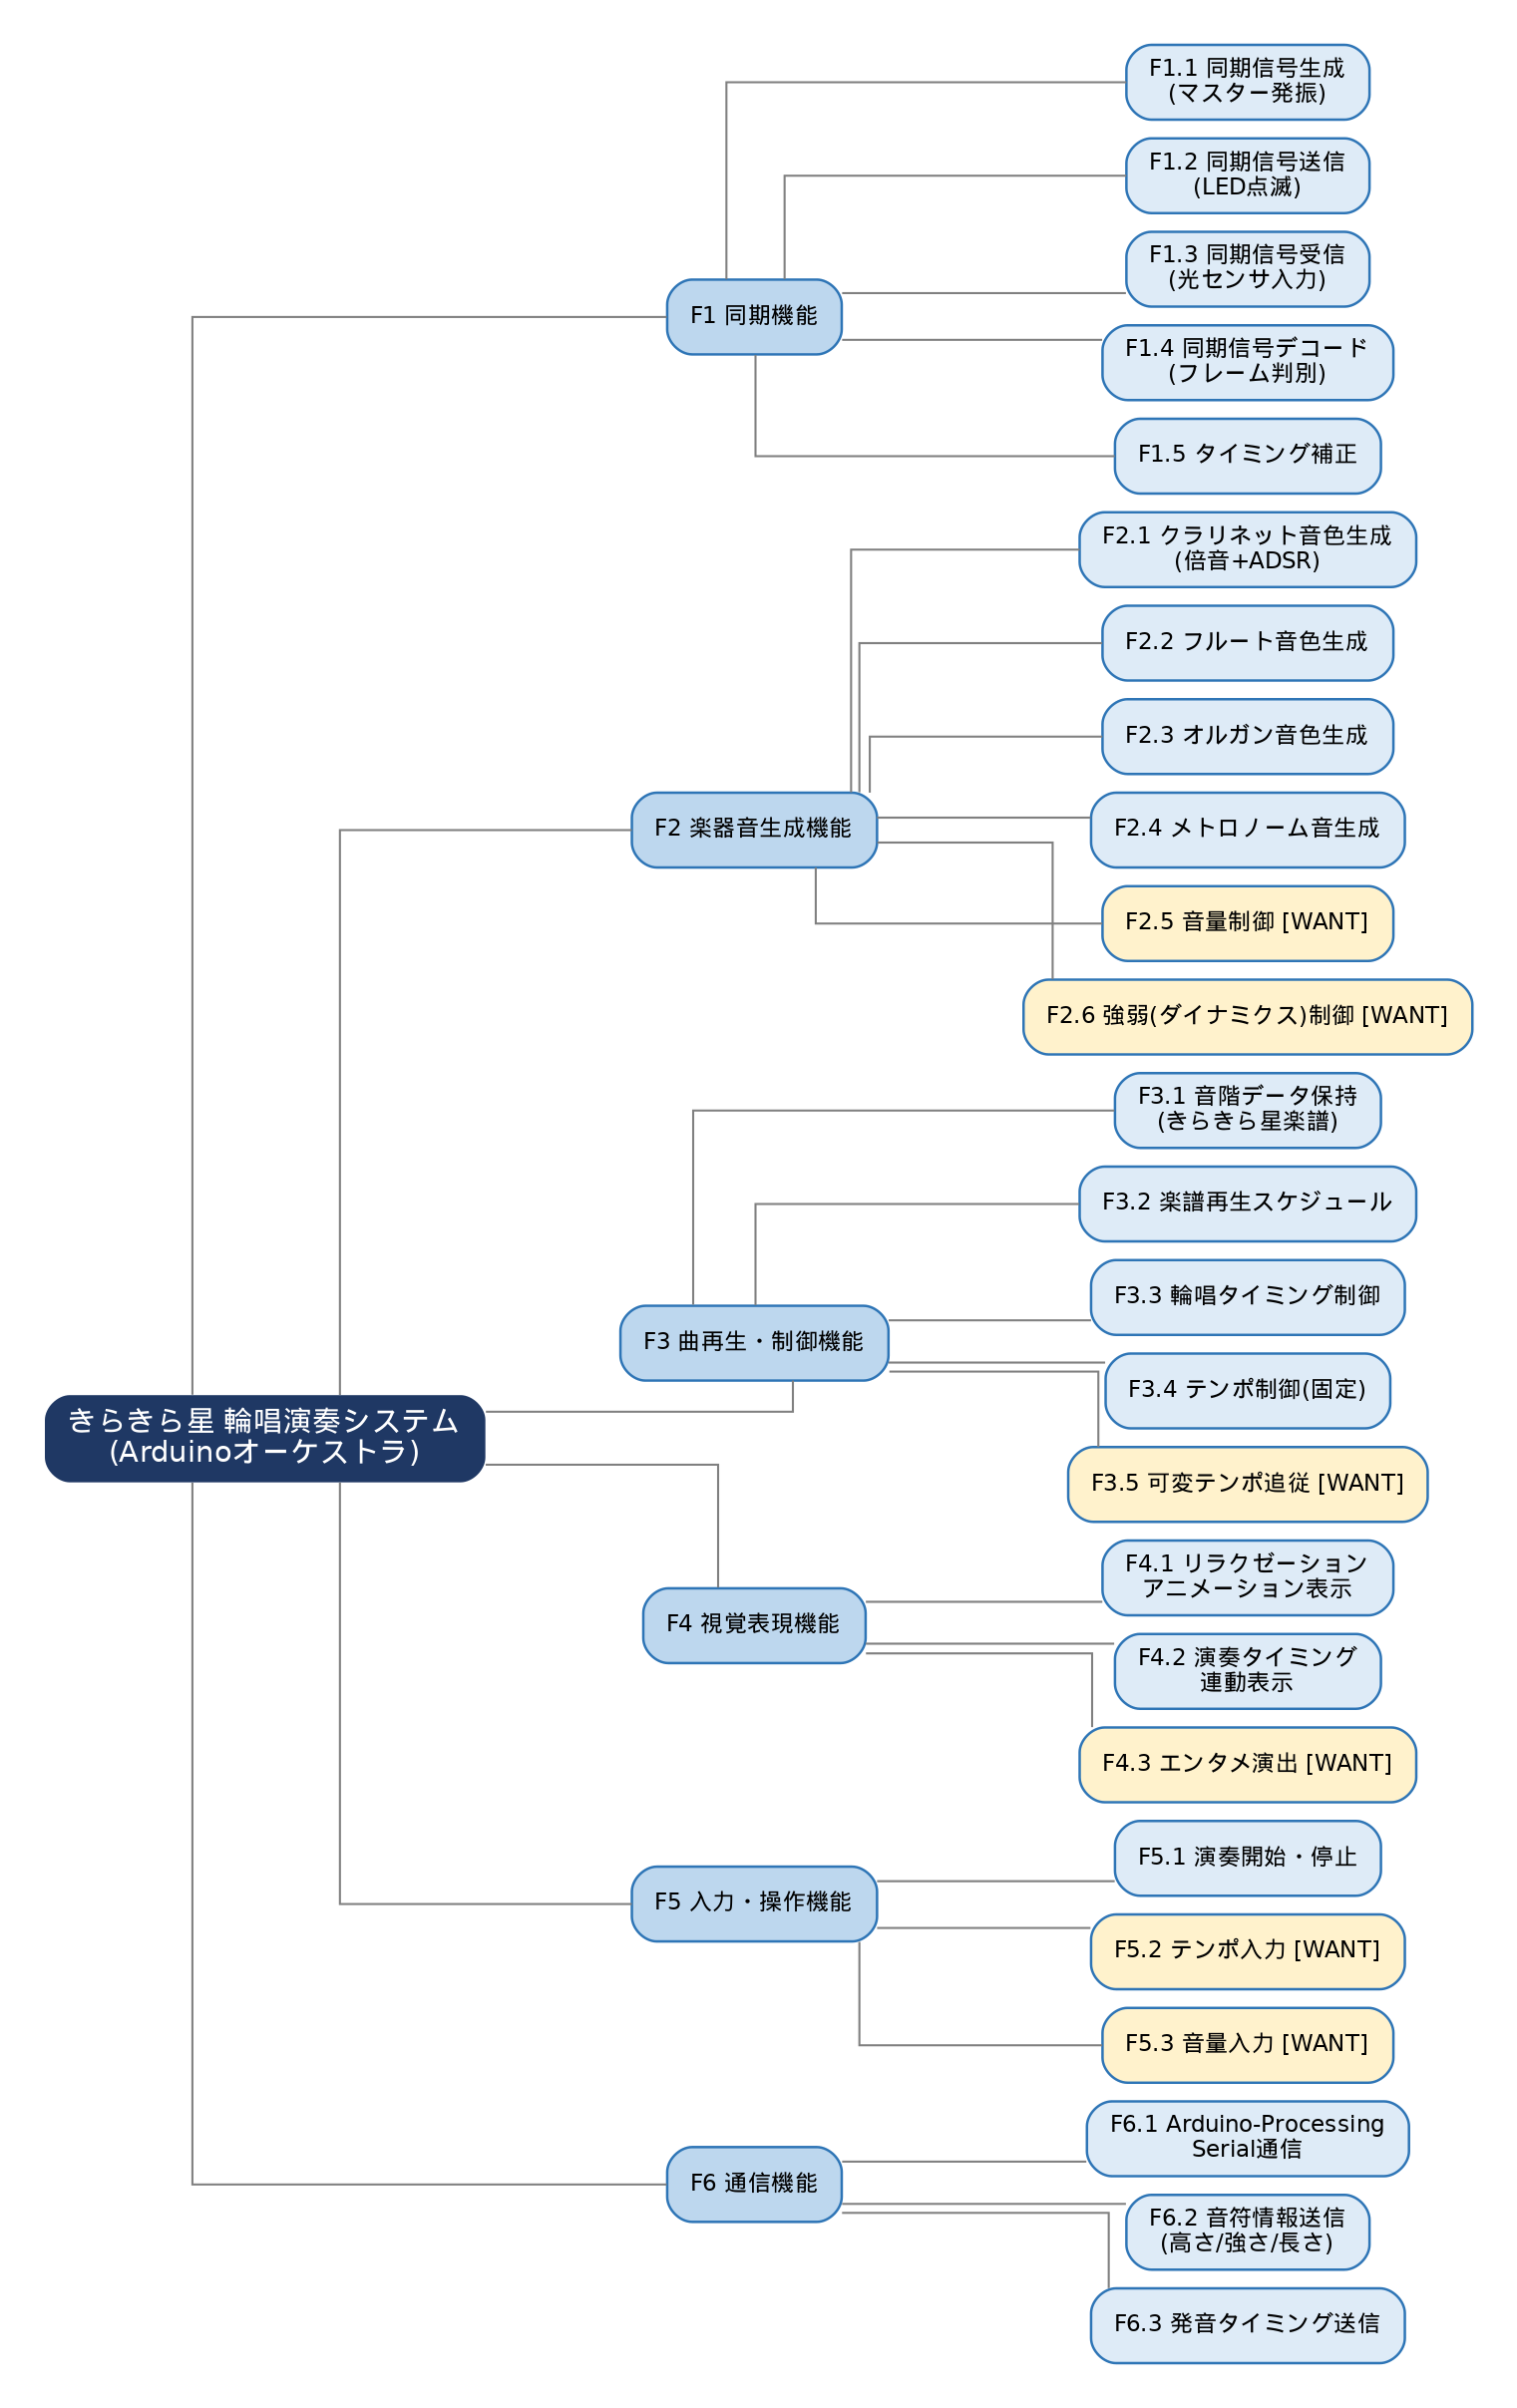
\includegraphics[width=0.85\textwidth]{fig/hck_fbs.png}
  \caption{FBS の原案}
  \label{fig:fbs}
\end{figure}

\subsubsection*{PBS}
\begin{figure}[H]
  \centering
  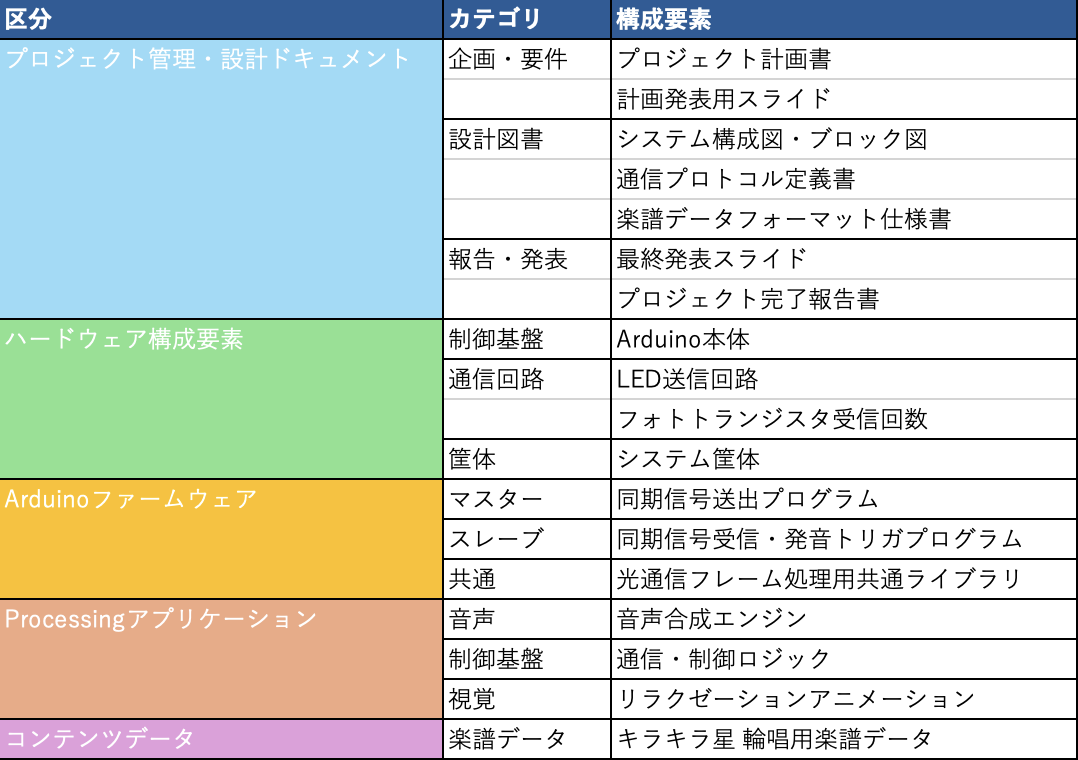
\includegraphics[width=0.85\textwidth]{fig/hck_pbs.png}
  \caption{PBS の原案}
  \label{fig:pbs}
\end{figure}

\begin{description}
  \item[ToDo / アクション] 各項目にぬけもれがないかを検査する
  \item[次回検討事項] FBS・PBS の確認・修正・確定
\end{description}

%-------------------------------------------------------------------
\subsection*{議題④：WBS と役割分担の原案}

\begin{figure}[H]
  \centering
  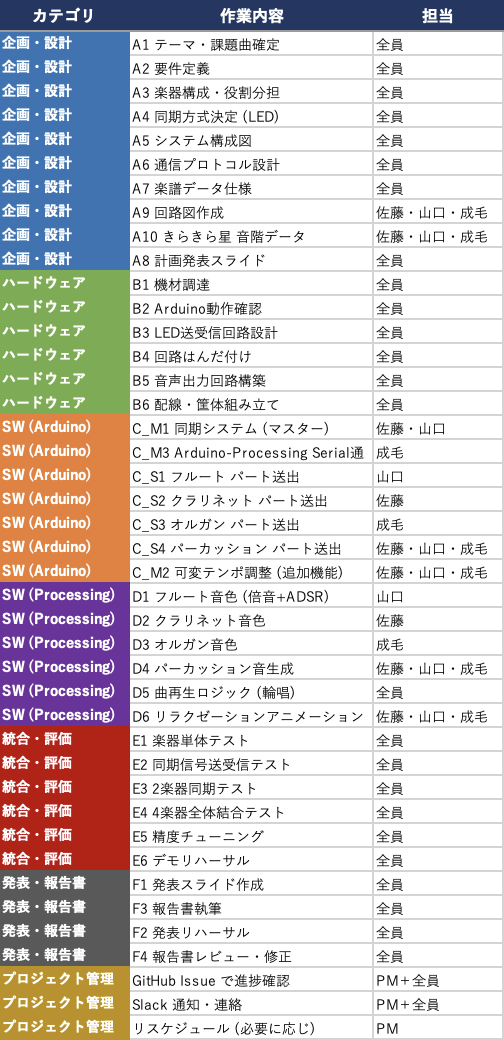
\includegraphics[width=0.6\textwidth]{fig/hck_wbs.png}
  \caption{WBS と役割分担の原案}
  \label{fig:wbs}
\end{figure}

\begin{description}
  \item[ToDo / アクション] 無茶な割り振りになっていないか，ぬけもれがないかを検査する
  \item[次回検討事項] WBS の確認・修正・確定
\end{description}

%-------------------------------------------------------------------
\subsection*{議題⑤：個人ごとの次回の役割の決定}

\noindent\textbf{輪唱曲：}キラキラ星

\vspace{2mm}
\noindent\textbf{担当楽器：}
\begin{center}
\begin{tabular}{ll}
  \toprule
  楽器 & 担当者 \\
  \midrule
  フルート & 山口汐里 \\
  クラリネット & 佐藤夏美 \\
  オルガン & 成毛海人 \\
  メトロノーム & 山口汐里，佐藤夏美，成毛海人 \\
  \bottomrule
\end{tabular}
\end{center}

\vspace{4mm}
\begin{description}
  \item[ToDo / アクション]~
    \begin{itemize}
      \item 2年生：担当楽器の詳細設計を作成
      \item 3年生：全体のシステムの構成を決定する
    \end{itemize}
  \item[次回検討事項] 設計の確認とレビュー
\end{description}

%-------------------------------------------------------------------
\section*{4. 次回予定}
\begin{tabular}{ll}
  \toprule
  日時・場所 & 2026年4月29日（水）・731教室 \\
  議題       & 詳細設計のすり合わせ \\
  \bottomrule
\end{tabular}

\end{document}
